\chapter[Bespreking]{Bespreking}
\label{chap_bespreking}

\section{Inhoud hoofdstuk ``Bespreking''}

Dit hoofdstuk zal uit de meeste onderdelen bestaan. Hier wordt het volledig gepresteerde werk beschreven, inclusief korte theoretische beschrijving (indien relevant. 
Vervolgens volgt een gedetailleerde beschrijving van hoe je tot het eindproduct bent gekomen, welke problemen je bent tegengekomen, hoe je ze hebt opgelost, etc.

%De titel van dit hoofdstuk zal meestal bestaan 'Bespreking [titel]' waarbij je een (kortere) werktitel neemt van je project, bijvoorbeeld: "Bespreking CRM project" of "Bespreking super-geleidende voltaische cel"

Dit hoofdstuk mag enkel flarden computer-code bevatten. Volledige source-code kan eventueel als appendix toegevoegd worden indien relevant en enkel met toestemming van de promotor.

Mogelijke onderdelen kunnen onder andere zijn:
\begin{itemize}
  \item Inleiding probleem (bestaand onderzoek/producten) 
  \item Functionaliteit van eigen product (algemeen overzicht)
  \item Architectuur van eigen product
  \item Bespreking aparte componenten/blokken (problemen + oplossingen)
  \item Bespreking werking van componenten samen
\end{itemize}


\section{\LaTeX voorbeelden}

\subsection{Refereren}

Het is mogelijk om met enkele eenvoudige commando's binnen uw tekst te refereren naar chapters, sections of figuren. 

Zo beschrijven we in hoofdstuk \ref{chap_besluit} op pagina \pageref{chap_besluit} wat we verwachten van een goed besluit en hebben we op pagina \pageref{fig_voorbeeld1} een voorbeeldfiguur geplaatst.  

Op pagina \pageref{eq:polynoom} staat een voorbeeld van een wiskundige formule.

De rode kaders zijn steeds klikbaar, maar ze worden niet mee afgedrukt op papier.

\subsection{Bibliografie}

Om te verwijzen naar een boek, artikel, website of een andere nuttige bron maken we gebruik van de bibliografie.
Het opnemen van artikels in de bibliografie geeft de persoon die uw tekst leest de mogelijkheid om meer informatie op te zoeken als er bepaalde zaken zijn die niet volledig worden uitgewerkt of toegelicht binnen uw scriptie.
De gegevens die in de bibliografie terecht komen worden uit het bestand ``bibliografie.bib'' gehaald. 

Om een nieuw item aan de bibliografie toe te voegen moet je dus twee zaken doen:

\begin{enumerate}
 \item De benodigde informatie toevoegen aan het .bib bestand
 \item Ergens binnen uw tekst verwijzen naar dit item met het ``cite'' commando.
\end{enumerate}

Hier is een voorbeeld van een verwijzing naar de bibliografie \cite{GridCast2} en dit is er ook \'e\'en \cite{gridrm}.

Ook hier zijn de groene kaders weer klikbaar en worden ze niet mee afgedrukt op papier.

De inhoud van de bibliografie zou vergelijkbaar moeten zijn met de informatie die je op onderstaande website kan vinden.

Harvard Referencing for Electronic Sources, \url{http://www.lc.unsw.edu.au/onlib/ref_elec1.html#elec10}



\subsection{Afbeeldingen}

Als je afbeeldingen invoegt, denk er dan aan dat deze voldoende van kwaliteit moeten zijn.

In afbeelding \ref{fig_voorbeeld1} zie je een afbeelding met een te lage resolutie. Afbeelding \ref{fig_voorbeeld2} ziet er al beter uit omdat deze figuur een hogere resolutie heeft.

Bij inzoomen of bij afdrukken zal figuur \ref{fig_voorbeeld3} toch nog iets hoger van kwaliteit zijn omdat dit een vectori\"ele afbeelding is. 
Standaard is ondersteuning voor .pdf en .eps vectorafbeeldingen voorzien.

\begin{center}
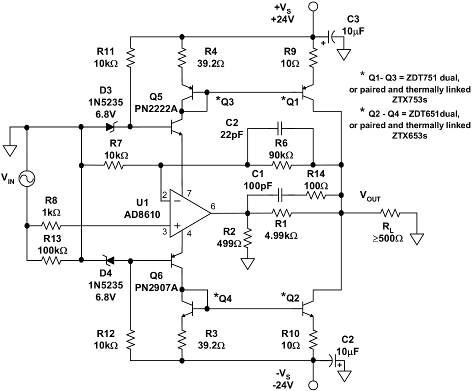
\includegraphics[width=0.95\textwidth]{figures/chap2/schema.png}
\captionof{figure}[Schema met een te lage resolutie22]{Schema met een te lage resolutie\label{fig_voorbeeld1}}
\end{center}

\begin{center}
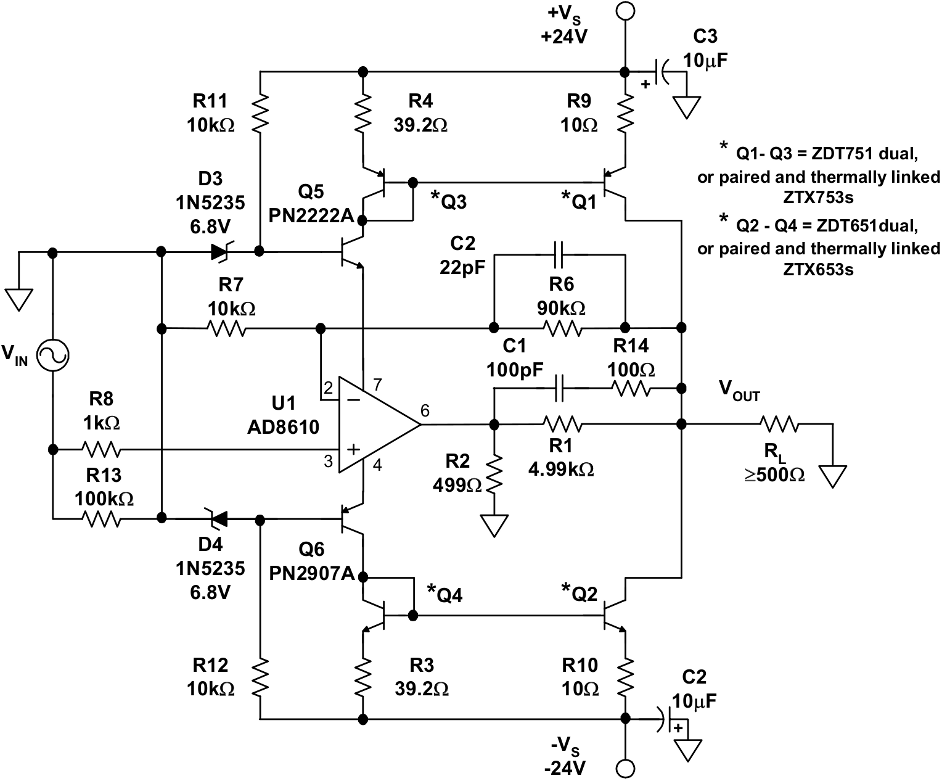
\includegraphics[width=0.95\textwidth]{figures/chap2/schema2.png}
\captionof{figure}[Schema met een hogere resolutie]{Schema met een hogere resolutie\label{fig_voorbeeld2}}
\end{center}

\begin{center}
\includegraphics[width=0.95\textwidth]{figures/chap2/schema2.pdf}
\captionof{figure}[Schema als een vectori\"ele afbeelding]{Schema als een vectori\"ele afbeelding\label{fig_voorbeeld3}}
\end{center}

\subsection{Tabellen}

De meest elementaire tabel geeft het volgende resultaat:

\begin{tabular}{ l c r }
  1 & 2 & 3 \\
  4 & 5 & 6 \\
  7 & 8 & 9 \\
\label{eenvoudige tabel}
\end{tabular}

Meer geavanceerde tabellen zijn iets moeilijker om te defini\"eren, maar als je op internet zoekt naar andere voorbeelden, die je kan overnemen en aanpassen zodat je bekomt wat je in gedachten had.

Een tabel met redelijk veel tekst die gecentreerd wordt weergegeven.

\begin{center}
    \begin{tabular}{ | l | l | l | p{5cm} |}
    \hline
    Day & Min Temp & Max Temp & Summary \\ \hline \hline
    Monday & 11C & 22C & A clear day with lots of sunshine.  
    However, the strong breeze will bring down the temperatures. \\ \hline
    Tuesday & 9C & 19C & Cloudy with rain, across many northern regions. Clear spells 
    across most of Scotland and Northern Ireland, 
    but rain reaching the far northwest. \\ \hline
    Wednesday & 10C & 21C & Rain will still linger for the morning. 
    Conditions will improve by early afternoon and continue 
    throughout the evening. \\
    \hline
    \end{tabular}
\label{tb:Xname}
\end{center}

Een iets complexere tabel die aan de linkerrand van de pagina wordt weergegeven.

\begin{flushleft}
\begin{tabular}{|l|l|l|}
\hline
\multicolumn{3}{|c|}{Team sheet} \\
\hline
Goalkeeper & GK & Paul Robinson \\ \hline
\multirow{4}{*}{Defenders} & LB & Lucus Radebe \\
 & DC & Michael Duberry \\
 & DC & Dominic Matteo \\
 & RB & Didier Domi \\ \hline
\multirow{3}{*}{Midfielders} & MC & David Batty \\
 & MC & Eirik Bakke \\
 & MC & Jody Morris \\ \hline
Forward & FW & Jamie McMaster \\ \hline
\multirow{2}{*}{Strikers} & ST & Alan Smith \\
 & ST & Mark Viduka \\
\hline
\end{tabular}
\end{flushleft}

\subsection{formules}

De mogelijkheden om formules in te voegen zijn \'e\'en van de sterkste punten van \LaTeX. 
Het vraagt in het begin wat moeite om de syntax onder de knie te krijgen, maar door intelligent gebruik te maken van de ``alternative text'' velden van wikipedia kan je heel snel formules opstellen.
(alle formules die je op Wikipedia terugvindt zijn namelijk ook met latex commando's geschreven.

Onderstaande formules geven een voorbeeld. Deze formules hebben ook een label, en ze worden automatisch genummerd, bijgevolg kan je er ook in je tekst op een dynamische manier naar verwijzen.

Voorbeeld: ``De Wet van Amp\`ere met Maxwell-correctie staat uitgeschreven in formule \ref{eq:maxwell} op pagina \pageref{eq:maxwell}.''

\begin{equation} \label{eq:polynoom}
x^2 - 5 x + 6 = 0
\end{equation}

\begin{equation} \label{eq:maxwell}
\oint_{\partial S} \mathbf{H} \cdot \mathrm{d}\mathbf{l} = I_{f,S} + \frac {\partial \Phi_S(\mathbf D)}{\partial t} 
\end{equation}

Je kan ook binnen een lopende tekst een formule toevoegen. Dit doe je door uw formule tussen twee dollartekens te plaatsen zoals ik hier doe $i \hbar {\partial \over \partial t} \Psi(x,\,t)= -{\hbar^2  \over 2m} {\partial^2 \over \partial x^2} \Psi(x,\,t)+ V(x)\Psi(x,\,t)\,$. Het is niet mogelijk om naar deze formule te verwijzen omdat er geen label aan werd toegekend.


\subsection{Packages}
Om extra functionaliteit toe te voegen aan het standaard \LaTeX systeem kan de gebruiker packages toevoegen. Dit is in die sjabloon reeds gedaan in het header.tex bestand.

Als je zelf extra packages wil toevoegen, doe dit dan steeds in overleg met je promotor. Sommige packages kunnen namelijk voor te grote veranderingen van de opmaak van het document zorgen.


\subsubsection{TODO}

Deze package laat het snel toevoegen van inline opmerkingen toe.
Het plaatsen van een opmerking gebeurt met het ``TODO[tekst]'' commando.
De tekst tussen [..] wordt opgenomen in het .pdf bestand en er wordt een apart .TODO bestand aangemaakt. 
In dit bestand krijg je een compact overzicht van alle ``todos'' in het volledige document.

\TODO[voorbeeld van een todo]

Deze package heeft drie mogelijk modi:

Standaard modus: weergaven van TODO zoals in bovenstaand voorbeeld
\begin{verbatim}
 \usepackage[final]{sty/TODO}
\end{verbatim}

Final modus: als er nog een todo in de tekst staat zal dit een error geven zodat je niet per ongeluk een ``final'' document kan afgeven met de TODO label er nog in.
\begin{verbatim}
 \usepackage[final]{sty/TODO}
\end{verbatim}

Silent modus: in deze modus worden de TODO label onderdrukt. 
Je kan dus een propere tekst genereren zonder al de TODO te moeten wissen of in commentaar te zetten. 
Dit kan nuttig zijn om een propere tussentijdse versie van uw scriptie aan te maken.
\begin{verbatim}
 \usepackage[silent]{sty/TODO}ackage 
\end{verbatim}







\subsection{Lijsten}

Voorbeeld met kleine interlinie:

\begin{enumerate*}
 \item Eerste element
 \item Tweede element
 \item Derde element
\end{enumerate*}

Voorbeeld met grotere interlinie:

\begin{enumerate}
 \item Eerste element
 \item Tweede element
 \item Derde element
\end{enumerate}


\subsection{Titels}

short title uitleggen

\subsection{Spellingscontrole}

editor afhankelijk

\section{Taalgebruik}

Spatie tussen eenheid en grootheid voor SI eenheden: \url{http://www.eng-tips.com/viewthread.cfm?qid=111559}
